%%%%%%%%%%%%%%%%%%%%%%%%%%%%%%%%%%%%%%%%%
% Academic Title Page
% LaTeX Template
% Version 2.0 (17/7/17)
%
% This template was downloaded from:
% http://www.LaTeXTemplates.com
%
% Original author:
% WikiBooks (LaTeX - Title Creation) with modifications by:
% Vel (vel@latextemplates.com)
%
% License:
% CC BY-NC-SA 3.0 (http://creativecommons.org/licenses/by-nc-sa/3.0/)
% 
% Instructions for using this template:
% This title page is capable of being compiled as is. This is not useful for 
% including it in another document. To do this, you have two options: 
%
% 1) Copy/paste everything between \begin{document} and \end{document} 
% starting at \begin{titlepage} and paste this into another LaTeX file where you 
% want your title page.
% OR
% 2) Remove everything outside the \begin{titlepage} and \end{titlepage}, rename
% this file and move it to the same directory as the LaTeX file you wish to add it to. 
% Then add \input{./<new filename>.tex} to your LaTeX file where you want your
% title page.
%
%%%%%%%%%%%%%%%%%%%%%%%%%%%%%%%%%%%%%%%%%

%----------------------------------------------------------------------------------------
%	PACKAGES AND OTHER DOCUMENT CONFIGURATIONS
%----------------------------------------------------------------------------------------

\documentclass[11pt]{article}

\usepackage[utf8]{inputenc} % Required for inputting international characters
\usepackage[T1]{fontenc} % Output font encoding for international characters
\usepackage{graphicx}
\usepackage{mathpazo} % Palatino font
\usepackage[legalpaper,margin=0.9in] {geometry}
\usepackage{fancyhdr}
\usepackage{float}

\setcounter{tocdepth}{4}
\setcounter{secnumdepth}{4}


\pagestyle{fancy}
\fancyhf{}
\lhead{\textsc{University of Regina}}
\rhead{\textsc{Software Systems Engineering}}
\cfoot{\thepage}

\begin{document}

%----------------------------------------------------------------------------------------
%	TITLE PAGE
%----------------------------------------------------------------------------------------

\begin{titlepage} % Suppresses displaying the page number on the title page and the subsequent page counts as page 1
	\newcommand{\HRule}{\rule{\linewidth}{0.5mm}} % Defines a new command for horizontal lines, change thickness here
	
	\center % Centre everything on the page
	
	%------------------------------------------------
	%	Headings
	%------------------------------------------------
	
	\textsc{\Huge University of Regina}\\[1.5cm] % Main heading such as the name of your university/college

	\textsc{\Large ENSE 477: Software Capstone Project}\\[0.5cm]
	
	\textsc{\Large Software Systems Engineering}\\[0.5cm] % Major heading such as course name
	
	
	
	
	%------------------------------------------------
	%	Title
	%------------------------------------------------
	
	\HRule\\[0.4cm]
	
	{\Huge\bfseries Workshop Enterprise Resource Planning Suite System and Object Design Document}\\[0.4cm] % Title of your document
	
	\HRule\\[1.5cm]
	
	%------------------------------------------------
	%	Author(s)
	%------------------------------------------------
	
	\begin{minipage}[t]{0.4\textwidth}
		\begin{flushleft}
			\large
			\textsc{Authors}\\
			Jonathan Wells\\
			\textsc{200328640}\\ % Your name
			\large
			Konstantin Kharitonov\\
			\textsc{200354502} % Supervisor's name
		\end{flushleft}
		
	\end{minipage}
	~
	\begin{minipage}[t]{0.4\textwidth}
		\begin{flushright}
			\large
			\textsc{Supervisor}\\ % Supervisor's name
			Karim Naqvi\\
			M.A.Sc., P.Eng.\\
		\end{flushright}
	\end{minipage}
	
	% If you don't want a supervisor, uncomment the two lines below and comment the code above
	%{\large\textit{Author}}\\
	%John \textsc{Smith} % Your name
	%------------------------------------------------
	%	Logo
	%------------------------------------------------
	
	\vfill\vfill\vfill\vfill
	
\includegraphics[width=0.7\textwidth]{UR.png}\\[2cm] % Include a department/university logo - this will require the graphicx package
	 

	%------------------------------------------------
	%	Date
	%------------------------------------------------
	
	\vfill\vfill\vfill % Position the date 3/4 down the remaining page
	
	{\large\today} % Date, change the \today to a set date if you want to be precise
	
	%----------------------------------------------------------------------------------------
	
	\vfill % Push the date up 1/4 of the remaining page
	
\end{titlepage}

%----------------------------------------------------------------------------------------

%----------------------------------------------------------------------------------------
%Table of Contents %

\newpage 
\tableofcontents
%-------------------------------------------------------------------------------------

%-------------------------------------------------------------------------------------
%Table of Figures % 
\newpage
\listoffigures

%-------------------------------------------------------------------------------------

\newpage
\section{Introduction}
The Workshop Enterprise Resource Planning Suite is an administrative overview and task management software designed for the University of Regina's on-campus engineering workshop. It is the primary workshop for campus for engineering students and administration, handling projects ranging from small in shop fixes to large scale capstone projects. This ERP is design to be the primary management tool used for the workshop, handling all day-to-day data for the shop. The ERP manages all incoming workorders, which are submissions by the student and/or faculty member detailing the specific request of the project they need the workshop for. All workorders are submitted, viewed and processed through this web application. As well, this system handles the project management by tracking the time of the billable and non-billable hours spent in the workshop. The third main feature of the application is the ability to manage the inventory of the shop, with the ability to search and find all the necessary data for a particular item in the workshop. With these features, the ERP is designed to become the primary source of data relating to the workshop and its activities. 

\subsection{Background}
Previous to the design of the ERP, the engineering workshop primarily stored all workorder data physically. All workorders were submitted in person on workorder forms, which are then stored into filled binders for recording purposes. All workorders ever submitted are kept in these binders and since they are filled out by hand, there are no copies made. Workorders, previous to this program, have not been copied.

\subsection{Purpose}
This system was designed to replace the previous methods of workorder, time, and inventory tracking, centralizing all aspects into one powerful application that can be accessed online. Workorders currently must be submitted via paper form directly to the workshop during its operating hours. The form must then be reviewed by the workshop manager and if accepted, future meetings are scheduled. All workorders submitted are then stored physically in binders, which date back to the opening of the workshop. All materials and inventory are also stored physically. This project intends to automate all workorders and have then be submitted and archived electronically. As well, the system is intended to track all scopes of projects, ranging from small miscellaneous tasks to larger scale projects in such a fashion that the workshop manager can schedule them effectively in advance. 
\subsection{Scope}
ERP is designed as a Web API, such that it is run in browser and is able to be accessed from any computer with a sufficient internet connection. It will be a local application that will be primarily accessed by the workshop manager, who is this project's main client. Secondary clients include faculty and staff that wish to submit workorders over the ERP suite. The primary client is the only one intended to have full control of all features of the ERP suite. 
\newline
{\setlength{\parindent}{0cm}

The ERP Suite currently is planned to be exclusive to the engineering workshop based on its design as of the completion of this capstone project, as future work on this project will require a redesign to be re-purposed for future clients. The ideal future client for this program is for machine and workshop owners with a staff less than 50.  

\newpage

\section{Design Overview}
A general overview of the ERP application, and how those features interact with each other during use. 

\subsection{General Overview}

The ERP is designed as a web application that the workshop manager, the main client of the program, can access the workshop's system from any computer using a web browser. The program in a web API, which connects to a remote database containing the workshop's data. The databases are hosted locally at the University of Regina, such that when used in the shop, information can accessed quickly and efficiently without having to deal with external server connections. 
\newline
{\setlength{\parindent}{0cm}

When a student or faculty member submits a workorder, it appears as a new item in the workorders page on the workshop manager's window. Each newly submitted workorder will be flagged as a new item, visually showing its status and that it requires attention. When a workorder is added to the system's calendar via the time tracking option, the system will flag its status to say that it is in progress, with the current estimated completion date included. Workorders that pass the current deadline will be flagged as being behind schedule. As well, the workshop manager can also flag any specific workorder as incomplete or cancelled on any workorders that have not been fully completed due to any particular restraints.
\newline
{\setlength{\parindent}{0cm}

In the time tracking section, the workshop manager has access to all currently submitted time entries, showcased in a calendar. Further display options are available such that the user can view the entries in a daily, weekly or monthly format. The entries are first split into two main categories, billable and non-billable time entries. These entries showcase what time was spent working on workorder projects for different clients, and what was spent doing other activities, such as small and/or miscellaneous fixes and builds. Each section is further broken down, with billable time showcasing exactly which project was worked on for how long. With this information, the workshop manager can then bill the student or faculty member for the right amount of work. 
\newline
{\setlength{\parindent}{0cm}

For the inventory section, the workshop manager has access to all of the materials and their respective data that is currently stored in the inventory table. Each entry has its own identifier, the price of which the material was last purchased for, information regarding the vendor who sells the product and any other relevant information. 

\subsection{Assumptions and Constraints}
For the web API to function, a connection to the internet and a modern browser to run the application. As is designed currently, the software is to be primarily used for the University of Regina, as the program has access to the university's financial services. Currently, the ERP suite is not designed for mobile use and should be used mostly on a computer. 

\newpage

\section{System Architecture}
This sections outlines the ERP suite and the program's design.


\subsection{Logical View}
The project is split into two main categories for development; the frontend and the backend. The following diagram showcases the details of the interface and their following subcategories. 
\begin{figure}[h]
	\centering
	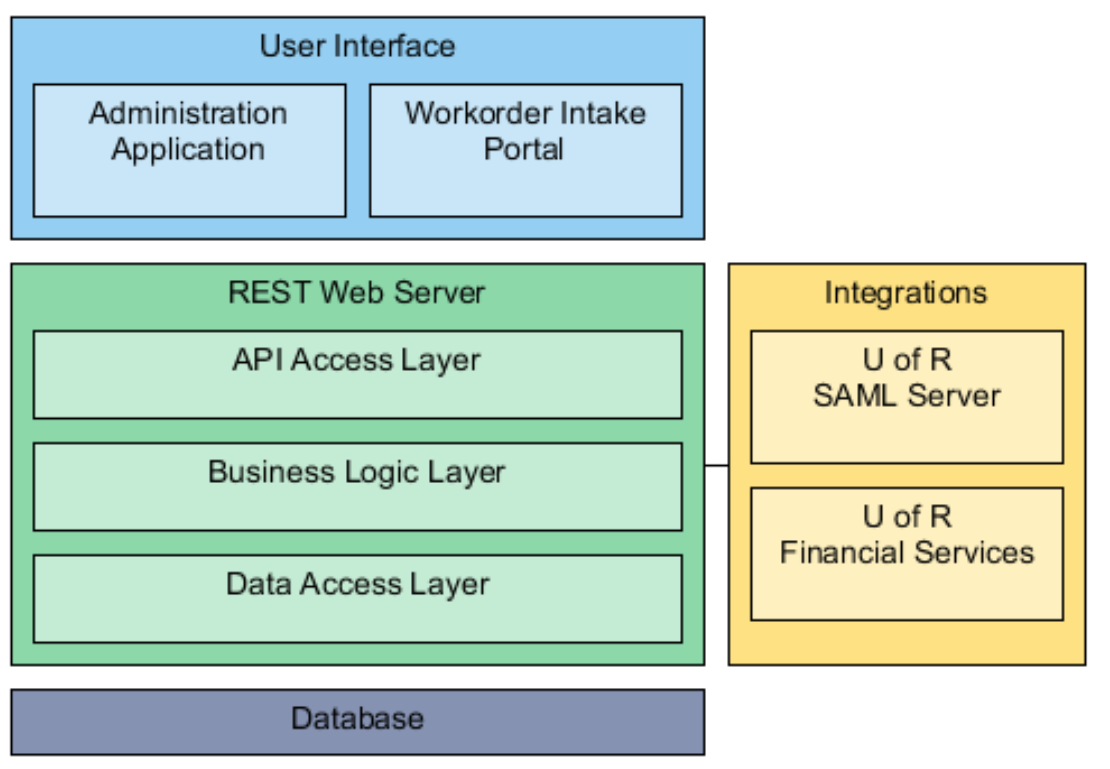
\includegraphics[width=3in]{front-back.png}\\
	\caption{Categories of the ERP Suite}
	\label{fig:tobias}
\end{figure}
\newline

On the front end, the client, who has the most control over the entire application. When the client log into the system upon start up, they have access to the main page displaying all necessary data for the particular day. In progress workorders, upcoming meetings and other related data can be quickly viewed. Clicking on a particular issue will navigate to a more in detailed view of the project. On the left side bar, the client can then access each particular section. 
\newline
{\setlength{\parindent}{0cm}

The first section is the Workorders page, where all workorders stored in the database can be accessed. Search and filtering options are available for the client when trying to locate specifics. Each workorder, displayed in a table with all necessary information, can be viewed, edited or deleted. When viewed in a closer look, tat particular workorder page is loaded, displaying all relevant information, including reference id, materials currently associated in the order, and all dates that apply. 
\newline
{\setlength{\parindent}{0cm}

The second section accessible by the left navigational bar is the time tracking feature, where the workshop manager can access the full calendar view of every time entry into the system, whether it is billable and non-billable hours. 

\subsection{Hardware Architecture}
Currently the application is a centralized system, with the client's operating machine and the server hosting the workshop's databases to be in the same location, thus allowing for the system to have a secure connection based on the university's internet. The type of server hosting the backend of the project is a REST web server, allowing the program to operate in a stateless environment, allowing the freedom of the application to transfer data to and from the database. This server is constructed using ASP.NET and entity framework, primarily written in the C\# language.   


\section{Data Design}
\section{External Interface Design}

\end{document}


